\section{A Competent Policy Still Fails Under Displacement}
\label{sec:competent}

\paragraph{The checkpoint is competent (E0).} The full action-expert fine-tune reaches $37/50=74\%$ clean success on the position-disciplined grid, with every task succeeding on at least one seed (per-task range $20$--$100\%$; median successful rollout length $104$ steps). This clears our pre-registered strong-checkpoint bar ($\geq 65\%$) and rules out the objection that the effect appears only in a weak $30$--$40\%$ policy. For comparison, a parameter-efficient (LoRA) fine-tune of the same backbone plateaus at $36$--$38\%$ regardless of learning rate; only the full action-expert recipe yields a competent policy (\cref{sec:emergence,sec:appendix}).

\paragraph{Displacement drives the reach to the canonical prior (E1r).} We run the full reach-field grid ($50$ pairs $\times$ $\{$clean $+$ $4$ magnitudes $\times$ $4$ cardinal directions$\}=850$ rollouts; $37$ clean-success pairs enter the primary set). At the headline $50$\,mm displacement, the clean-conditioned primary endpoint yields a median $\cossim(\ev,-\dv)=0.759$ with task-cluster bootstrap CI $[0.693,0.847]$, a signed projection of $0.98$, and $68\%$ of endpoints closer to the canonical location $\Cv$ than to the displaced object $\Tv$. All four pre-registered criteria pass. \cref{fig:cloud} shows the geometry directly: in the displacement frame, the endpoints of a competent policy form a cloud centered at $\Cv$, not at the object $\Tv$. A projection of $0.98$ means the endpoint barely moves as the object is displaced---the policy reaches as though the object were still at its training location. The effect replicates on an independent training seed (seed-1: $50$\,mm clean-conditioned median $\cossim(\ev,-\dv)=0.844$ at $76\%$ clean success, overlapping CI), so it is not a single-seed artifact (\cref{sec:limitations}).

\begin{figure}[t]
\centering
\begin{subfigure}{0.46\textwidth}
  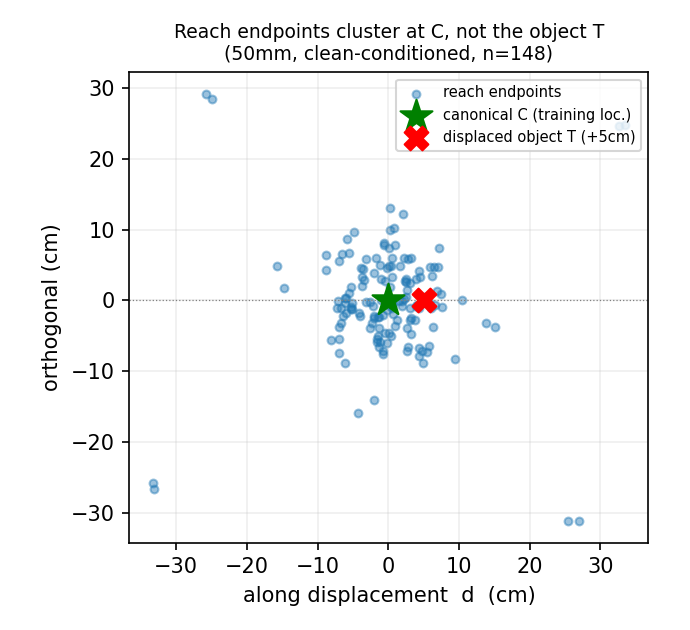
\includegraphics[width=\linewidth]{figures/fig_endpoint_cloud.png}
  \caption{Endpoints cluster at $\Cv$, not $\Tv$ ($50$\,mm).}
  \label{fig:cloud}
\end{subfigure}\hfill
\begin{subfigure}{0.46\textwidth}
  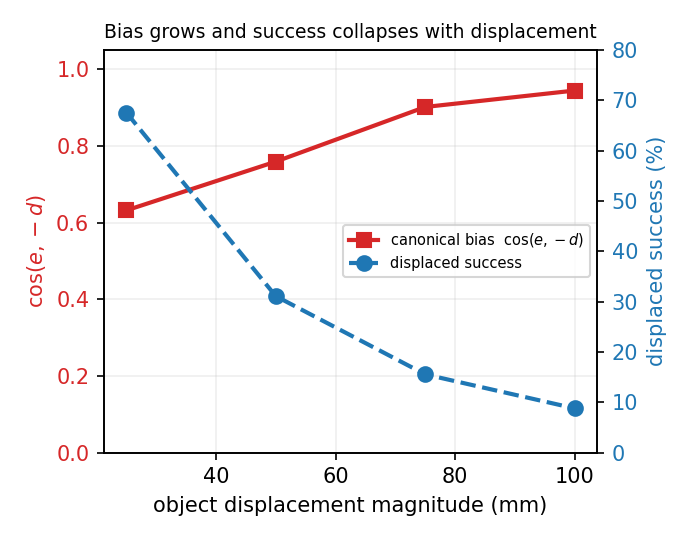
\includegraphics[width=\linewidth]{figures/fig_magnitude.png}
  \caption{Bias rises and success collapses with magnitude.}
  \label{fig:magnitude}
\end{subfigure}
\caption{\textbf{Reach-field on the competent ($74\%$) SmolVLA checkpoint.} (a) Clean-conditioned reach endpoints $\Ev$ in the displacement frame ($x$ along $\dv=\Tv-\Cv$); green star $=$ canonical/training location $\Cv$, red cross $=$ displaced object $\Tv$. The endpoint error is $\ev=\Ev-\Tv$, and our statistic $\cossim(\ev,-\dv)>0$ means the reach points back toward $\Cv$ (the canonical prior). (b) The alignment $\cossim(\ev,-\dv)$ increases monotonically with displacement while displaced success collapses.}
\label{fig:e1r}
\end{figure}

\paragraph{The bias scales and predicts failure.} The alignment increases monotonically with displacement magnitude---median $\cossim(\ev,-\dv)$ of $0.63$, $0.76$, $0.90$, $0.94$ at $25$, $50$, $75$, $100$\,mm---and the fraction closer to canonical rises from $61\%$ to $86\%$ (\cref{fig:magnitude}). In lockstep, displaced success collapses from $68\%$ at $25$\,mm to $31\%$, $16\%$, and $9\%$, despite $74\%$ clean success. The larger the displacement, the more the reach ignores it, and the more the episode fails. The endpoint error points toward the canonical prior \emph{despite a fresh post-displacement observation}: the policy is not acting on stale pixels, but on a location it has learned to aim at.
